\section{Accidents barotraumatiques}

\begin{frame}{Principe général}
  \begin{columns}[c]
    \begin{column}{0.5\textwidth}
      \begin{itemize}
        \item Les volumes de gaz se \textbf{compressent} à la descente,
              se \textbf{dilatent} à la remontée (loi de Mariotte).
        \item Si l’air ne peut pas circuler librement, il y a un \textbf{risque de lésion} des tissus.
        \item On parle de \textbf{barotraumatismes}.
      \end{itemize}
    \end{column}
    \begin{column}{0.5\textwidth}
      \centering
      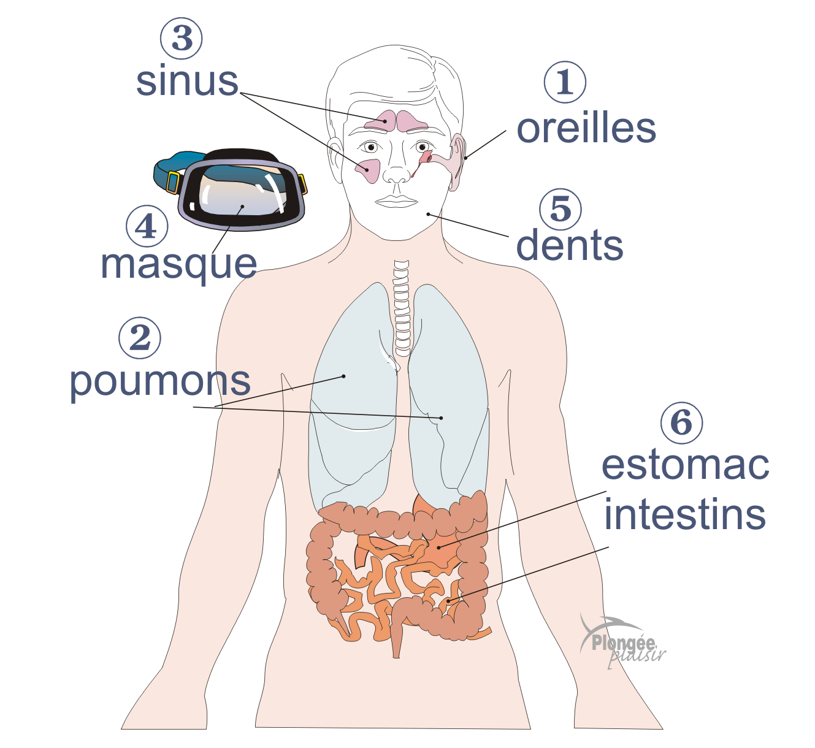
\includegraphics[width=\textwidth]{images/les-6-accidents-barotraumatique}
    \end{column}
  \end{columns}
\end{frame}

\begin{frame}{Plaquage de masque}
  \begin{itemize}
    \item À la descente, l’air dans le masque se \textbf{comprimes}.
    \item La jupe agit comme une \textbf{ventouse} sur le visage et les yeux.
    \item Risques : rougeurs, douleurs, troubles de la vue.
  \end{itemize}
  \begin{block}{Prévention}
    \begin{itemize}
      \item \textbf{Souffler par le nez dans le masque} à la descente.
      \item S’assurer que le masque est bien ajusté mais pas trop serré.
    \end{itemize}
  \end{block}
\end{frame}

\begin{frame}{Dents}
  \begin{block}{Dents}
    \begin{itemize}
      \item Cavités d’air dans une dent mal soignée.
      \item Douleurs à la descente ou à la remontée, risque d’\textbf{éclatement de la dent}.
      \item Prévention : suivi \textbf{régulier chez le dentiste}, arrêter la plongée en cas de douleur persistante.
    \end{itemize}
  \end{block}
\end{frame}

\begin{frame}{sinus}
  \begin{columns}[c]
    \begin{column}{0.45\textwidth}
        \begin{block}{Sinus}
          \begin{itemize}
            \item Cavités osseuses communiquant avec les fosses nasales.
            \item Obstruction $\Rightarrow$ impossibilité d’égaliser la pression.
            \item Douleurs violentes, parfois \textbf{saignements}.
            \item Prévention : ne pas plonger enrhumé, ne jamais forcer, consulter un ORL en cas de problème.
          \end{itemize}
        \end{block}
      \end{column}
    \begin{column}{0.5\textwidth}
      \centering
      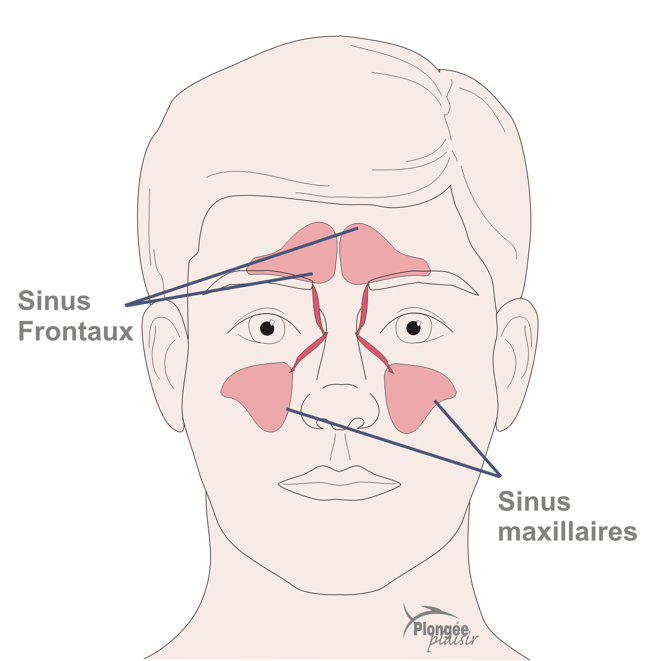
\includegraphics[width=0.9\textwidth]{images/barotraumatisme-sinus}
    \end{column}
  \end{columns}
\end{frame}

\begin{frame}{Oreilles}
  \begin{columns}[c]
    \begin{column}{0.45\textwidth}
      \begin{itemize}
        \item Tympan situé entre oreille externe et oreille moyenne.
        \item À la descente : pression extérieure augmente, tympan repoussé vers l’intérieur.
        \item Si on n’égalise pas : \textbf{douleur}, risque de \textbf{rupture du tympan}.
      \end{itemize}
    \end{column}
    \begin{column}{0.5\textwidth}
      \centering
      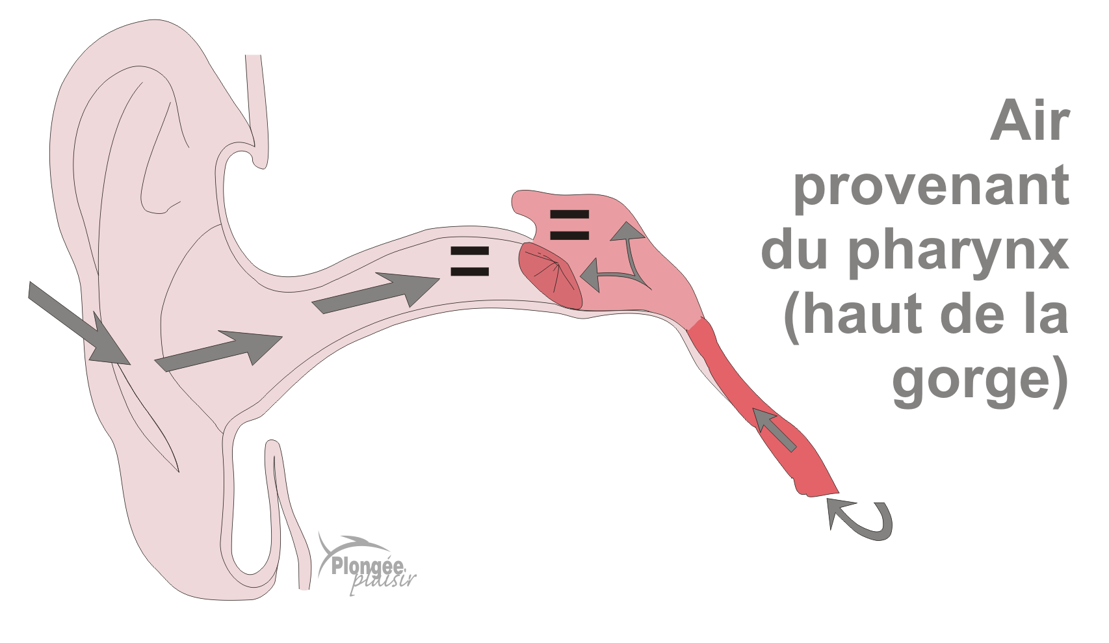
\includegraphics[width=0.9\textwidth]{images/barotraumatisme-oreille}
    \end{column}
  \end{columns}
\end{frame}

\begin{frame}{Manœuvre de Valsalva}
  \begin{block}{Manœuvre de Valsalva}
    \begin{itemize}
      \item Se pincer le nez, bouche fermée, et \textbf{souffler doucement}.
      \item L’air passe par la trompe d’Eustache et rétablit l’équilibre de pression.
      \item À faire \textbf{régulièrement à la descente}, avant la douleur.
      \item \alert{Ne jamais faire de Valsalva à la remontée}.
    \end{itemize}
  \end{block}
  
  \vspace{0.2cm}

  \begin{alertblock}{Attention - conduite à tenir}
    \begin{itemize}
      \item Si, à la descente, une \textbf{douleur survient}, remonter de
            \textbf{quelques mètres} puis redescendre doucement.
      \item \alert{Ne jamais insister}.
      \item Si la douleur persiste : \textbf{consulter un ORL}.
    \end{itemize}
  \end{alertblock}
\end{frame}

\begin{frame}{Coliques du scaphandrier}
  \begin{itemize}
    \item Gaz dans le tube digestif : fermentation des aliments, boissons gazeuses, air avalé.
    \item À la remontée : dilatation des gaz, douleurs abdominales.
  \end{itemize}
  \begin{block}{Prévention}
    \begin{itemize}
      \item Éviter les \textbf{féculents lourds} et les \textbf{boissons gazeuses} avant la plongée.
      \item Manger léger et adapté.
    \end{itemize}
  \end{block}
\end{frame}
